\documentclass{article} 
\usepackage[T1]{fontenc}
\usepackage[utf8]{inputenc} % Para acentos
\usepackage{graphicx}       % Para imágenes
\usepackage{geometry}       % Para ajustar márgenes
\usepackage{listings}  
\usepackage{hyperref}       % Para enlaces clicables
\usepackage{titling}        % Para subtítulo en \maketitle

\hypersetup{
    colorlinks= true,
    linkcolor= blue,
    urlcolor=blue
}
\geometry{margin=1.5cm}


\title{Análisis y especificaciones de requisitos}

\author{Iván Alfaya Pérez}

\date{\today}


\newcommand{\subtitle}{Proyecto: Aplicacion Movil de gestor de usuarios} % Subtítulo

\posttitle{\par\vspace{0.5cm}\large \subtitle\end{center}\vskip 0.5cm} 
\begin{document}

\maketitle

% Imagen debajo del título
\begin{figure}[h!]
    \centering
    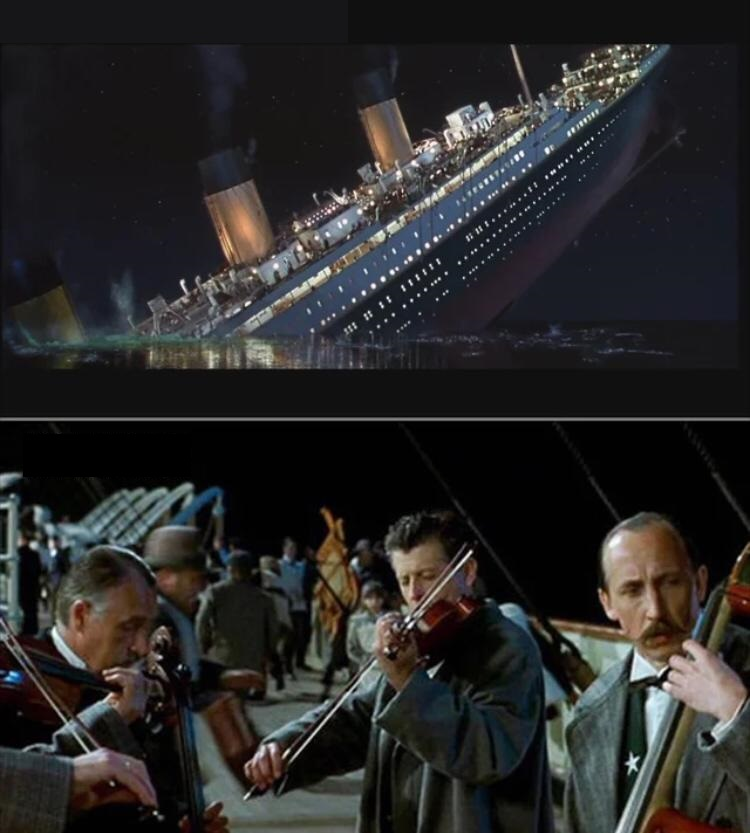
\includegraphics[width=0.7\textwidth]{img1.jpg}
\end{figure}

\clearpage 

\tableofcontents % Tabla de contenido
\clearpage 

\section{Descripcion del Problema}
Aquí va el contenido de la introducción.

\section{Metodología}
Detalles sobre la metodología.


\section{Resultados}
Resultados obtenidos.

\section{Conclusiones}
Conclusiones finales.

\end{document}
